% 1987 年上海卷第四题：三棱锥 S-ABC
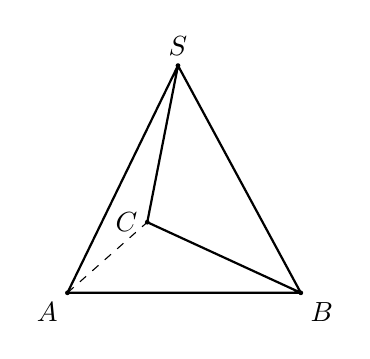
\begin{tikzpicture}[scale=0.78,>=stealth]
  \coordinate (S) at (1.8,3.7);
  \coordinate (A) at (0,0);
  \coordinate (B) at (3.8,0);
  \coordinate (C) at (1.3,1.15);
  \draw[thick] (S)--(A) (S)--(B) (S)--(C) (A)--(B) (B)--(C);
  \draw[dashed] (A)--(C);
  \fill (S) circle (1.1pt) node[above] {$S$};
  \fill (A) circle (1.1pt) node[below left] {$A$};
  \fill (B) circle (1.1pt) node[below right] {$B$};
  \fill (C) circle (1.1pt) node[left] {$C$};
\end{tikzpicture}
